%
% This file is part of ICTP RegCM model.
% Copyright (C) 2011 ICTP Trieste
% See the file COPYING for copying conditions.
%

\section{The Gforge site}

A new welcoming home for the RegCM Community has been built with the help
of Italian National Research Council CNR Democritos Group on the e-science
Lab E-Forge web site:

\vspace{0.5cm}
\begin{tabular}{|c|}
\hline
{\bf https://gforge.ictp.it/gf/project/regcm} \\
\hline
\end{tabular}
\vspace{0.5cm}

\begin{figure}[h!]
\caption{The Gforge site}
\centering
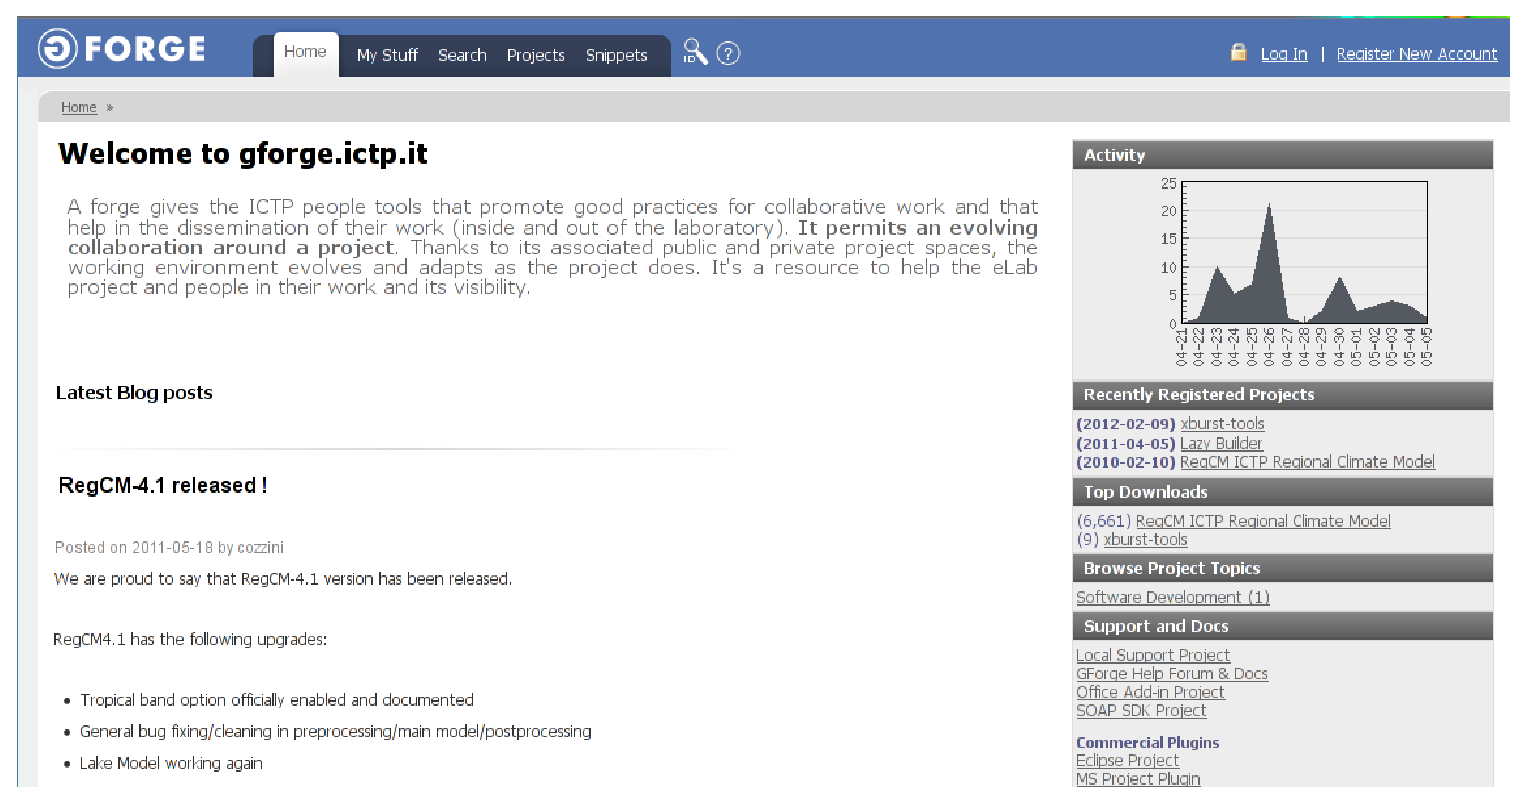
\includegraphics[width=12cm]{gforge}
\end{figure}

On this site you have access with a simple registration to a friendly
bug tracking system under the {\em tracker} link, allowing the users to
post problems and bugs they discover.

It allows posting also of files to give you the opportunity to provide as
much information as possible about the environment the model is running at
your institution, helping us better understand and solve efficiently your
problems.

Help us grow the model to fit your requirements, giving the broader user
community the benefit of a valuable tool to do better research.
